\section{Unüberwachtes Lernen}

\subsection{Neuronale Merkmalskarten}
Übernehme Idee der Lokalität aus dem biologisches Vorbild. (siehe Skript Folie 145ff. für genaue Beschreibung)

\paragraph{Problem}
Man hat sehr viele Datenpunkte in einem hochdimensionalen Merkmalsraum. Außerdem sind häufig zu Beginn der Analyse noch nicht alle Datenpunkte bekannt. Vor allem sind \textbf{keine} Lehrersignale vorhanden.

\subsection{Reduktion der Datenpunkte}
\paragraph{Ziele}
\begin{itemize}
    \item Repräsentation der Eingabedaten bestimmen
    \item prototypische Repräsentationen sollen berechnet werden 
    \item Ähnliche Daten werden durch gleichen Prototyp repräsentiert
    \item Regionen mit hoher Datendichte sollen durch mehrere Prototypen repräsentiert werden
    \item erstellen einer Kartenstruktur, benachbarte Neuronen/Prototypen sollen durch ähnliche Eingaben aktiviert werden
\end{itemize}

\subsection{Kompetetives neuronales Netz}

\begin{figure}[h]
    \centering
    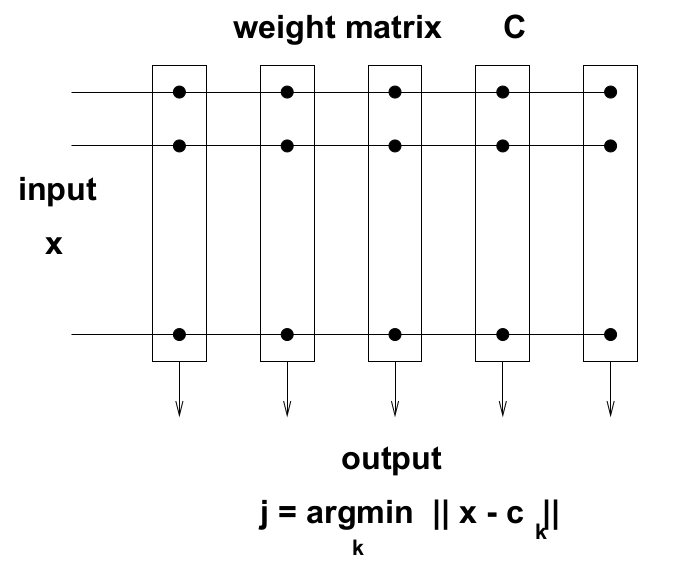
\includegraphics[width=.33\textwidth]{img/NeuroLernregel/kompNetz.png}
    \caption{Architektur komp. Netz}
    \label{ch_lern_upstart}
\end{figure}

\subsubsection{Distanz vs. Skalarprodukt zur Gewinnerdetektion}
Die euklidische Norm ist gegeben durch
\begin{equation*}
    \norm{x}_2 = \sqrt{\langle x,x \rangle}
\end{equation*}
Damit gilt für den Abstand von $x,y\in\mathbb{R}^n$
\begin{equation*}
    \norm{x-y}_2^2 = \langle x-y,x-y \rangle = \langle x,x\rangle -2\langle x,y\rangle + \langle y,y\rangle = \norm{x}_2^2 - 2\langle x,y \rangle + \norm{y}_2^2
\end{equation*}
Dann gilt für die Gewinnerdetektion bei der Eingabe $x$ unter den durch $c_1,\dots,c_k$ und $\norm{c_i}_2=1$ gegebenen Neuronen 
\begin{equation*}
    j^* = \operatorname{argmax}_i \langle x,c_i \rangle \quad \Longleftrightarrow \quad j^* = \operatorname{argmin}_i \norm{x-c_i}_2
\end{equation*}

\subsection{Kohonen's selbstorganisierende Karte}
\begin{figure}[h]
    \centering
    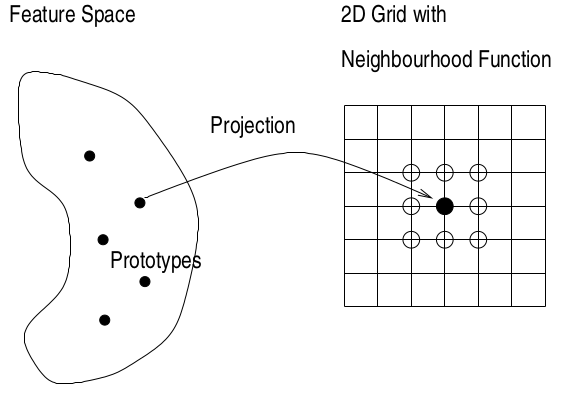
\includegraphics[width=.33\textwidth]{img/NeuroLernregel/SOM.png}
    \caption{Darstellung der Kohonen Karte}
    \label{ch_lern_SOM}
\end{figure}
\paragraph{Ziele}
\begin{itemize}
    \item Berechnung von Prototypen im Merkmalsraum, also $c_i \in \mathbb{R}^d$, die die gegebenen Daten $x\in\mathbb{R}^d$ gut repräsentieren
    \item Nachbarschaftserhaltende Abbildung der Prototypen $c_i\in\mathbb{R}^d$ auf Gitterpositionen $g$ auf ein Gitter im $\mathbb{R}^2$
\end{itemize}

Es kann damit die Kohonen Lernregel formuliert werden
\begin{equation*}
    \Delta c_{ij} = l_t N_t(g_j,g_{j^*})\cdot(x-c_j)
\end{equation*}

Hierbei ist $j^*$ der Gewinner, $N_t$ eine Nachbarschaftsfunktion, $g_j$ die Gitterposition des j-ten Neurons auf der Karte und $l_t$ und $\sigma_t$ sind trainingszeitabhängige Lernraten bzw. Nachbarschaftsweitenparameter. Diese beiden Parameter sollten bei steigender Trainingszeit t gegen $0$ konvergieren.\\
Eine mögliche Nachbarschaftsfunktion ist gegeben durch $N_t(g_j,g_{j^*} = \exp{(-\frac{\norm{g_j-g_{j^*}}_2^2}{2\sigma_t^2})}$

\subsection{Kohonen Lernalgorithmus}
Gegeben ist der Input $X = \{x_1,\dots,x_M\}\subset \mathbb{R}^d$

\begin{enumerate}
        \item Wähle $r,s\in\mathbb{N}$ eine Clusterzahl $k=rs\in\mathbb{N}$, eine Lernrate $l_t>0$ und eine Nachbarschaftsfunktion $N$ und maximale Lernepochenzahl $N_{max}$. $t=0$
        \item Initialisiere die Prototypen $c_1,\dots,c_k \in\mathbb{R}^d$, diese bilden Matrix $C\in\mathbb{R}^{k\times d}$
        \item Jeder Prototyp auf genau eine Gitterposition $g_i \in \{1,\dots,r\}\times\{1,\dots,2\}$
        \item \texttt{\textbf{repeat}\\
            Wähle $x\in X$ und $t=t+1$\\
            $j^* = \operatorname{argmin}_i\norm{x-c_i}$ (winner detection)\\
            \textbf{for all j:}\\
            $c_j = c_j + l_tN_t(g_j,g_{j^*}(x-c_j)$ (update)}
        \item bis $t\geq N_{max}$    
\end{enumerate}
Siehe Skript Folie 161 ff. für Anwendungsbeispiel.


\subsection{Kompetetives Lernen}
Gegeben ist der Input $X = \{x_1,\dots,x_M\}\subset \mathbb{R}^d$
\begin{enumerate}
    \item Wähle Clusterzahl $k\in\mathbb{N}$ und eine Lernrate $l_t>0$ und $N$. $t=0$
    \item Initialisiere Prototypen $c_1,\dots,c_k\in\mathbb{R}^d$ bilden dann Matrix $C\in\mathbb{R}^{k\times d}$
    \item \texttt{\textbf{repeat}\\
        Wähle $x\in X$ und $t=t+1$\\
        $j^* = \operatorname{argmin}_i\norm{x-c_i}_2$ (winner detection)\\
        $c_{j^*} = c_{j^*} + l_t(x-c_{j^*})$ (winner update)}
    \item bis $t\geq N$
\end{enumerate}

\todo[inline]{einfügen der Notizen aus der Vorlesung}

\subsection{k-means Clusteranalyse}
Der Datenpunkt $x\in\mathbb{R}^d$ wird dem nächsten Clusterzentrum $c_{j^*}$ zugeordnet.
\begin{equation*}
    j^* = \operatorname{argmin}_j\norm{x-c_j}
\end{equation*}
Das Clusterzentrum wird dann angepasst
\begin{equation*}
    \Delta c_{j^*} = \frac{1}{|C_{j^*}|+1}(x-c_{j^*})
\end{equation*}
Vergleich zum kompetitiven lernen
\begin{equation*}
    \Delta c_{j^*} = l_t(x-c_{j^*})
\end{equation*}


\subsection{ART-Netzwerke (Adaptive-Resonanz-Theorie}
Im folgenden wird nur die Grundlegende ART1 Architektur. Auf dieser aufbauend gibt es verschiedene Erweiterungen ART2, ART3, FuzzyART und ARTMAP.\\
Bei ART-Netzen handelt es sich um kompetitive Netze. ART-Netze sind wachsende Netze. Die maximale Anzhal der Neuronen ist jedoch beschränkt.\\
Bei ART1-Netzen sind die Eingabedaten und die Gewichtsvektoren/Prototypen binäre Vektoren.

\subsubsection{ART1-Lernen}
\begin{itemize}
    \item Inputvektoren und Prototypen $\in\{0,1\}^d$
    \item es wird nur der Gewichtsvektor des Gewinnerneurons $c_{j^*}$ adaptiert
    \item ist Ähnlichkeit zwischen Input $x$ und Prototyp $c_{j^*}$ zu gering, so wird durch $x$ ein neuer Prototyp definiert und $c_{j^*}$ wird nicht verändert
    \item Ähnlichkeit wird durch Skalarprodukt $\langle x,c_j \rangle$ gemessen
    \item Schranke für Mindestähnlichkeit wird durch Vigilanzparameter bestimmt
    \item ist Ähnlichkeit größer als Schranke, so wird $c_{j^*}$ durch komponentenweises \textbf{AND} von $x$ und $c_{j^*}$ adaptiert
    \item maximale Anzahl an Neuronen wird vorgegeben
\end{itemize}

\paragraph{ART1-Algorithmus}
Der Eingabevektor $x_\mu \in \{ 0,1 \}^d$ mit $\mu=1,\dots,M$, die Gewichtsvektoren bzw. Prototypen sind gegeben durch $c_i\in \{ 0,1 \}^d$. Mit $\textbf{1} = (1,1,\dots,1)\in \{ 0,1 \}^d$ wird der Eins-Vektor bezeichnet. $k$ ist die Anzahl der maximal möglichen Neuronen. Durch $\norm{x}_1$ ist die Eins-Norm definiert, diese gibt die Anzahl der Einsen an. Durch $\rho\in[0,1]$ ist der Vigilanzparameter gegeben.\\

\begin{enumerate}
    \item \texttt{Wähle $k\in\mathbb{N}$ und $\rho\in[0,1]$}
    \item \texttt{Setze $c_i=\textbf{1}$ für alle $i=1,\dots,k$}
    \item \texttt{WHILE noch ein Muster $x$ vorhanden DO\\
        Lies $x$ und setze $I=\{1,\dots,k\}$\\
        REPEAT\\
        $j^* = \operatorname{argmax}_{j\in I}\frac{\langle x,c_j\rangle}{\norm{c_j}_1}$ (winner detection)\\
        $I = I \setminus {j^*}$\\
        UNTIL $I=\emptyset$ or $\langle x, c_{j^*} \rangle \geq \rho \norm{x}_1$\\
        IF $\langle x, c_{j^*} \rangle \geq \rho \norm{x}_1$\\
        THEN $c_{j^*} = x\wedge c_{j^*}$ (winner update)\\
        ELSE keine Bearbeitung von $x$
        }
    \item \texttt{END}
\end{enumerate}
Zunächst werden die Hyperparameter $k$ und $\rho$ gewählt. Es werden dann die Gewichtsvektoren zu $\textbf{1}$ initialisiert. Es wird dann der Prototyp mit der größten Ähnlichkeit zu $x$ gesucht und der jeweilige Prototyp dann aus der Menge entfernt. Ist die Ähnlichkeit höher als der Schwellwert $\rho \norm{x}_1$ wird der Prototyp angepasst. Ist dies nicht der Fall tritt der Fall der Leerenmenge ein und $x$ wird implizit zu einem neuen Prototypen.

\subsection{LVQ (Lernende Vektorquantisierung)}
Bei LVQ handelt es sich um überwachte Lernverfahren zur Musterklassifikation. Bei LVQ-Verfahren handelt es sich um heuristische kompetitive Lernverfahren.\\
Es wird die euklidische Distanz zur Berechnung der Ähnlichkeit verwendet. Im folgenden wird nur LVQ1 behandelt. Es gibt diverese Erweiterungen wie LVQ2, LVQ3 und OLVQ.

\subsubsection{LVQ1-Algorithmus}
Der Input ist gegeben durch $X = \{(x_1,y_1),\dots,(x_M,y_M)\}\subset\mathbb{R}^d\times\Omega$ dabei ist $\Omega=\{1,\dots,L\}$ eine endliche Menge von Klassen(-Labels).

\begin{enumerate}
    \item \texttt{Wähle Prototypenzahl $k$, eine Lernrate $l_t>0$ und N. Setze $t=0$
    \item \texttt{Initialisiere Prototypen $c_1,\dots,c_k\in\mathbb{R}^d$}}
    \item \texttt{Bestimme für jeden Prototypen $c_i$ die Klasse $\omega_i\in\Omega$}
    \item \texttt{REPEAT\\
        Wähle ein Paar $(x,y)\in X$ und setze $t=t+1$\\
        $j^*=\operatorname{argmin}_i \norm{x-c_i}$ (winner detection + class from nearest neighbor\\
        IF $\omega_{j^*} \neq y$ THEN $\Delta = -1$ ELSE $\Delta = 1$ (check if classification result is correct)\\
        $c_{j^*} = c_{j^*} = l_t\Delta(x-c_{j^*})$ (winner update)}
    \item UNTIL $t\geq N$    
    
\end{enumerate}
